\documentclass[runningheads]{llncs}

\usepackage[T1]{fontenc}
\usepackage{graphicx}
\usepackage{tabularx}

\usepackage{polyglossia}
\setmainlanguage{english}
\setotherlanguage{farsi}

% Define Arabic font
\newfontfamily\arabicfont[Script=Arabic]{Amiri}

%
\begin{document}
%
\title{Expanding Flicker30k: a Novel Dataset for Persian Language Captions}
%
%\titlerunning{Abbreviated paper title}
% If the paper title is too long for the running head, you can set
% an abbreviated paper title here
%
\author{Shima Baniadamdizaj\inst{1}\orcidID{0000-0003-1678-5108} \and
Alexander Breuer\inst{1} }
%
\authorrunning{Sh. Baniadamdizaj et al.}
% First names are abbreviated in the running head.
% If there are more than two authors, 'et al.' is used.
% 
\institute{Friedrich Schiller University Jena, Jena, Germany \\
\email{\{sima.bani, alex.breuer\}\@uni-jena.de}}
%
\maketitle              % typeset the header of the contribution
%
\begin{abstract}
Image captioning, the challenge of describing images through natural language, particularly benefits from deep learning techniques, necessitating substantial, diverse datasets. While existing datasets like Microsoft COCO and Flickr30k offer valuable resources, they are predominantly in English. The Expanding Flicker30k dataset fills this void for the Persian language. With manually curated captions averaging 13.3 words, the dataset captures various visual scenarios. By addressing the absence of Persian captioning resources, this paper contributes to both image captioning and cross-lingual research, fostering improved image understanding and language generation capabilities.
This paper presents a novel resource for Persian language image captioning. Built upon the Flickr30k dataset, the new collection comprises 51,000 captions corresponding to 10,200 distinct images, providing a crucial dataset for advancing image captioning research in the Persian language. Each picture has five captions in Persian, which helps overcome the lack of non-English captioning datasets and allows for detailed language analysis. The dataset includes columns for image names, comment numbers, Persian captions, and English translations, facilitating bilingual comparisons.

\keywords{Image Captioning in Persian \and Computer Vision \and Natural language processing \and image-to-text.}
\end{abstract}
%
%
%
\section{Introduction}
% \subsection{A Subsection Sample}
Image captioning refers to the automated process of describing the content of an image using natural language sentences. While humans can interpret images without explicit descriptions, machines struggle with the task of generating natural and informative captions. They need to understand the semantic relationships between objects in an image, their attributes, and the actions in order to generate accurate and coherent descriptions, which is an effortless task for humans. Additionally, machines need to translate these semantic relations into correct literature. For instance, a suitable caption for an image which has a train and people at a station, may involve describing people either boarding the train or waiting on the platform.

The prevalent methods employed for image captioning predominantly rely on deep learning techniques \cite{Karpathy2015,Vinyals2015,Xu2015,Luo2023}. Deep learning-based image captioning relies on extensive image datasets to train models effectively. The availability of a large volume of diverse images is crucial for capturing complex situations. Although there is a vast array of image sources available through television, the internet, news, and other platforms, the majority of these images lack accompanying descriptions. Various captioned image datasets, such as Microsoft COCO \cite{MSCOCO}, Flickr8k \cite{Flickr8k}, and Flickr30k \cite{Flickr30k}, offer valuable resources for training deep learning models in image captioning tasks. These datasets contain diverse images with human-generated captions, enabling the development of accurate and meaningful captioning models.

The discussed datasets consist of image captions in the English language. However, there exists a scarcity of large-scale image captioning datasets available for languages other than English. For instance, the Multi30k dataset \cite{Multi30k}, encompassing English-German captions. Translating existing English datasets into other languages offers an inexpensive approach for training models to generate non-English captions. Studies \cite{Xue,Zoph,Rosa} have specifically shown that employing translated datasets, rather than using originally annotated datasets in the target language, can adversely affect model performance.

In light of these considerations, there is a scarcity of available image captioning datasets specifically for the Persian language. However, to address this gap, we have developed a dataset based on the widely used Flickr30k dataset \cite{Flickr30k} for Persian language image captioning. To the best of our knowledge, this dataset represents the first proposed solution for the worldwide Image Captioning problem with Persian captions. The dataset consists of 10,180 image labels randomly selected from Flicker30k and manually captioned by different individuals. Each image is associated with five distinct reference descriptions. The average length of descriptions is 13.3 words, with a standard deviation of 5.5 words. Additionally, it should be noted that the Persian prepositions are considered as an independent word in this dataset and are separated from the next word by space.

This paper comprises five chapters, each vital to exploring Persian image captioning. Chapter 1 introduces the research and stresses the need for a dedicated dataset. Chapter 2 explores motivation, related works, and existing datasets, emphasizing the gap for a Persian dataset. Chapter 3 details dataset collection, annotation, and preprocessing. Chapter 4 presents experiments, discussions, and analyses. Chapter 5 concludes and outlines future prospects. This work contributes a resource for Persian language visual understanding and bridges the gap in image captioning research.

% Chapter 2
\section{Motivation and Related Works}
The machine's ability to perform image captioning has been greatly facilitated by the availability of large-scale annotated datasets. Some well known examples of such datasets in English language are Microsoft COCO \cite{MSCOCO}, Flickr8k \cite{Flickr8k} and Flickr30k \cite{Flickr30k}. Despite the existence of non-English image captioning datasets, such as Multi30k \cite{Multi30k} and VIST \cite{VIST} for English-German and English-Chinese captions, respectively, there is still a noticeable scarcity of Persian language datasets. The availability of large-scale captioning datasets specifically in Persian is limited, which presents a challenge for training models to generate captions in this language.

\subsection{English Captioned Datasets}
MS COCO (Microsoft Common Objects in COntext) \cite{MSCOCO} is an extensively used computer vision dataset. It contains a collection of over 164k images, sourced from diverse platforms. The dataset offers comprehensive annotations, including precise bounding boxes for object detection and segmentation masks. The training set consists of approximately 83k images, while the validation and test sets contain around 41k images each. Consequently, the average sentence length of the descriptions is approximately 10 words. The dataset is widely utilized in various computer vision tasks, including object recognition, scene understanding, and image captioning.

Flickr8k \cite{Flickr8k} is another notable computer vision dataset widely used in the field. It is specifically designed for image captioning tasks and consists of a diverse collection of 8k high-quality images sourced from the popular photo-sharing platform Flickr. Each image in the dataset is accompanied by five human-generated captions, providing rich textual descriptions of the visual content. The dataset aims to capture a wide range of scenes, objects, and activities, showcasing the diversity of real-world imagery. The Flickr8k dataset has become a resource for training and evaluating image captioning models, enabling researchers to develop algorithms that generate accurate and contextually relevant descriptions for images. The availability of Flickr8k has played a role in advancing the field of image captioning and in natural language understanding and computer vision.

In addition to the Flickr8k dataset, another notable dataset is the Flickr30k dataset. The Flickr30k \cite{Flickr30k} dataset is an extension of Flickr8k, with a larger collection of images and relevant captions. While Flickr8k comprises 8k images, Flickr30k consists of approximately 30k images, making it substantially larger in scale.Both datasets share similarities in terms of their origin, as they are sourced from the popular photo-sharing platform Flickr. They aim to represent diverse scenes, objects, and activities, capturing images in their natural context. Both datasets are accompanied by human-generated captions that provide textual descriptions of the visual content. However, the increased size of the Flickr30k dataset brings several advantages. The increased diversity of content enhances model robustness and generalization in computer vision tasks. The larger number of images in Flickr30k provides a wider representation of real-world scenarios and concepts. This enhanced coverage allows researchers to tackle more complex challenges in object recognition, scene understanding, and image captioning tasks. 

There is another dataset specifically created for the task of image captioning called ``Nocaps'' \cite{Nocaps}. The dataset contains a large-scale collection of images and their corresponding captions. It emphasizes novel and diverse scenes, aiming to expand the range of images and situations that captioning models can handle effectively. Each image in the Nocaps dataset is associated with multiple human-generated captions. The dataset has a total of 166,100 human-generated captionsfor 15,100 images for over 500 unique object classes. The images of this dataset are sourced from the Open Images V4 \cite{Openimages}. The Open Images V4 dataset is a publicly available dataset for large-scale multi-label and multi-class image classification tasks. The OpenImages dataset offers a diverse range of visual concepts, ensuring a comprehensive representation of real-world objects and scenes.The dataset comprises 1.9 million images depicting complex scenes.

Some of the image captioning datasets are provided for a specific case. For example, the VizWiz-Captions dataset \cite{VizWiz} is specifically designed to address the unique challenges faced by people with visual impairments in understanding visual content. The dataset contains approximately 31k images, each accompanied by a human-generated caption. 
There is an overlap of about 54\% between the VizWiz and MS COCO datasets in terms of the provided captions. The images and captions in the VizWiz-Captions dataset were collected through the VizWiz mobile application. This application enables visually impaired users to capture images and ask questions about the content.

The mentioned datasets have limitations, as they provide captions for only English speakers. This lack of other language representation shows the necessity of the development of image captioning datasets for non-English speakers. This will enable a more comprehensive and inclusive environment for advancing image captioning task, and provide a wider accessibility and applicability across different languages.

\subsection{Non-English Image Captioning Datasets}
As there is currently no specific Persian language image captioning dataset available, when discussing image captioning, the focus of this section is on non-English datasets instead of observing Persian ones. This shows the need for the development of Persian-specific datasets in the field of image captioning.

One of the well known examples of non-English image captioning datasets is the Multi30k dataset \cite{Multi30k}, which is a widely used benchmark dataset for image captioning and multimodal machine translation tasks.It is an extension of the Flickr30k dataset \cite{Flickr30k} and is aimed at generating English-German captions. Exactly like Flicker30k dataset, each image has five reference captions but this time in German. Researchers rely on Multi30k to benchmark and advance the performance of models in generating accurate and meaningful captions in both English and German languages.

There is a Korean Tourist Spot (KTS) \cite{Korean} which is a multiple modal dataset. It means that the dataset consists of images with textual descriptions, and additional metadata like hashtags and likes. This dataset is specifically tailored for studying Korean tourist spots and includes a total of 10 classes. The KTS dataset was collected from Instagram and followed by a preprocessing step. It comprises a substantial amount of data, with a total of 10k instances. Each of the 10 classes within the dataset is composed of 1k instances.

The ImageCLEF 2018 \cite{ImageCLEF2018} dataset's images and their corresponding captions extracted from biomedical articles on PubMed Central and contains 232,305 pairs of image and caption, which were divided into separate training and test sets. The training set consists of 222,305 pairs, and the test set contains 10,000 pairs. The dataset includes multiple languages commonly used in biomedical research, such as English, Spanish, German, French, etc.

\subsection{Persian Image Captioning Datasets}
Datasets such as MS COCO and Flickr have multiple unofficial versions available for various languages, but no Persian. The lack of a Persian language image captioning dataset highlights the need for developing datasets specifically designed for Persian in image captioning tasks. Considering both native and second language speakers, it is estimated that there are approximately 110 to 120 million Persian language speakers worldwide. This includes native speakers from Iran, Afghanistan, and Tajikistan, as well as second language speakers through education, migration, interest, or cultural affinity.

The collection of an image captioning dataset in Persian holds importance for several reasons. Developing an image captioning dataset in Persian, one of the widely spoken languages in the Middle East and Central Asia, addresses the need for natural language processing in this language for the Persian-speaking population and development in AI research. A Persian image captioning dataset opens doors for various practical applications, including content recommendation systems, image search engines, accessibility tools for visually impaired individuals, and language learning platforms which currently are not supporting this language.

Moreover, creating a Persian image captioning dataset promotes cultural preservation and representation. Persian culture encompasses a rich heritage of art, traditions, and historical landmarks. By focusing on images relevant to Persian culture and context, we capture the essence of Persian identity and contribute to preserving and showcasing its visual heritage. This dataset is valuable for documenting, educating about, and promoting Persian culture.

In conclusion, the collection of an image captioning dataset in Persian addresses the specific linguistic and cultural needs of the Persian-speaking community. It enables development in AI research, and contributes to the preservation and promotion of Persian cultural heritage. By undertaking this endeavor, we aim to bridge the language gap in how images are understood and make AI technologies more accessible and inclusive for everyone.

\section{Dataset Description}
The following section presents the detailed data collection and analysis procedures. The dataset comprises a collection of images that were exclusively sourced from Flickr30k \cite{Flickr30k}. This section focuses on detailing the process of data collection and labeling, specifically for Persian image captioning. The aim is to provide a comprehensive understanding of the procedure followed to gather the dataset.

To initiate the data collection process, various sources were explored to obtain a diverse range of images suitable for Persian image captioning. Special attention was given to selecting images that represented a broad spectrum of subjects, scenarios, and contexts, ensuring the dataset's comprehensiveness and inclusivity. There is one example from dataset in Fig.~\ref{fig1}. 

\begin{figure}[htbp]
\begin{center}
  \begin{minipage}[t]{0.3\textwidth} 
    \vspace{0pt}
    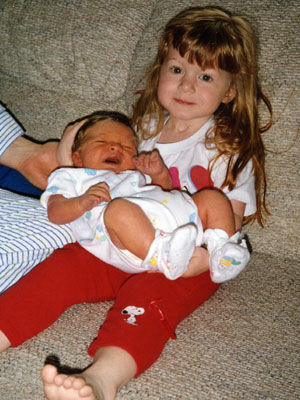
\includegraphics[width=\textwidth]{2656351.jpg}
  \end{minipage}
  % \hfill % Add space between the image and the table
  \begin{minipage}[t]{0.6\textwidth}
    % \vspace{-\baselineskip} % Remove vertical space before the table
    \vspace{0pt} % Remove vertical space before the table
    \begin{tabularx}{\linewidth}{|X|} \hline
      \begin{farsi} \arabicfont\small دختر جوانی با شلوار قرمز اسنوپی نوزاد بسیار کوچکی را در دامان خود نگه داشته است.\end{farsi} \\ 
      \hline
      \begin{farsi} \arabicfont\small دختر کوچک و مو قرمز نوزادی تازه در آغوش گرفته است.\end{farsi} \\ 
      \hline
      \begin{farsi} \arabicfont\small دختری کوچک روی کاناپه که نوزادی را در آغوش گرفته است.\end{farsi} \\
      \hline
      \begin{farsi} \arabicfont\small یک دختر جوان یک نوزاد گریان را در آغوش گرفته است.\end{farsi} \\
      \hline
      \begin{farsi} \arabicfont\small دختربچه ای که نوزادی را در آغوش دارد.\end{farsi} \\
      \hline
    \end{tabularx}
  \end{minipage}
  \caption{Example image from the dataset with relative captions.}
  \label{fig1}
    \end{center}
\end{figure}

\subsection{Image Collection}
This paper focuses on the collection and annotation of a dataset of images sourced from Flickr30k \cite{Flickr30k} which contains a diverse community of photographers and accordingly photos. Both amateur enthusiasts and seasoned professionals contribute to this platform, resulting in a rich and varied collection of photos. This feature ensures representation across a wide array of visual attributes. These sources were carefully chosen to ensure the availability of high-quality images aligned with the desired scope of the study.

Additionally, these selected images were carefully chosen to contain various situations and were annotated by human annotators same as the original dataset (Flicker30k). By using some of the images from the Flickr dataset, we enable multitask learning and transfer learning approaches for image captioning tasks involving two languages (English/ Persian).

\subsection{Annotation Procedure}
The annotators were instructed to describe the images using words or sentences that accurately depicted the content, focusing on the most important aspects of each image. Annotators fluent in Persian were asked to do a captioning task to ensure the captions accurately reflect the semantic meaning and context of the images, including grammar, syntax, and nuances. Each image in the dataset is annotated with five different captions. Although some captions may have similarities, they are entirely distinct. If duplicate captions were found for an image, one of them was removed, and the annotator was asked to provide a new caption.

To maintain consistency and enhance the overall quality of the dataset, a comprehensive annotation guideline was developed. This guideline provided clear instructions and specifications to the annotators, ensuring uniformity in the captioning process and minimizing variations in style and content. This step was crucial to facilitate the training of machine learning algorithms for automatic image captioning in the Persian language in exact terms. This involved organizing the selected images, collecting relevant metadata, and removing duplicates or any unessential content Through these steps, the dataset was carefully cleaned, standardized, and prepared for further analysis. 

To validate the quality of the captions, we asked evaluators to check some specific criteria. These criteria included checking if the caption accurately described the corresponding image, contained at least one word, is grammatically correct, and does not contain any foreign language or harmful content. 

As a result, by carefully following this data collection and captioning procedure, a robust dataset for Persian image captioning was created which provides a resource for training and evaluating machine learning models in the context of automatic image captioning in the Persian language. This dataset can potentially serve as a bilingual (English/ Persian) dataset for various tasks such as image captioning and image description.

\subsection{Content Analysis}
The captioning dataset yielded a total of 51000 captions for 10200 unique images, which means there are five different captions for each image. 
The dataset consists of four columns. The first column, ``image\_name'',
contains the name or number of each image from the Flickr30k image dataset. The images are in JPG format and maintain their original sizes from the Flickr dataset. The second column, ``comment\_number'', indicates the number of captions associated with each image, ranging from 0 to 4. Each image has five distinct captions. The third column, ``comment-fa'', stores the Persian comments for each image which is the main contribution of this paper. Finally, the last column, ``comment-en'', contains the English captions imported from the Flickr30k dataset.

As part of the dataset preprocessing, it is important to note that the ``comment-fa'' column does not contain non-Persian alphabet characters. Also, all numbers are written alphabetically rather than using digits. This consideration helps ensure consistent handling and maintain uniformity throughout the dataset. The Prefixes or suffixes are not counted as a word in this dataset for example \begin{farsi} \arabicfont\small "ها"\end{farsi} (plural sign), or \begin{farsi} \arabicfont\small "های"\end{farsi} (plural sign). But pre-positions and post-positions like \begin{farsi} \arabicfont\small "با"\end{farsi} (with), \begin{farsi} \arabicfont\small "از"\end{farsi} (from), or \begin{farsi} \arabicfont\small "و"\end{farsi} (and) are considered as a separate word and are counted. By these considerations the shortest caption length is two words and the longest one includes 77 words. The caption in the collected dataset with the longest length belongs to image number 207344485 (row 16052 in csv file, see Fig.~\ref{fig2}.a), containing 77 words, which is:

\begin{farsi}
\arabicfont\small
"مردی با یک شلوار قرمز و کلاه ایمنی با راه راه‌های سفید در کناره‌ها و یک پیراهن سفید و قرمز روی دوچرخه‌ای کوچک تنها با استفاده از دست‌هایش ایستاده است درحالی که پاهایش در هوا هستند مرد دیگری پیراهن آبی روشن با طرح های آبی تیره به تن دارد شلوار مشکی با نوارهای قرمز در کناره‌ها در همان نزدیکی ایستاده است و به مرد اول اشاره می‌کند و مجسمه کوچک یکی از هفت کوتوله را در دست دارد."
\end{farsi}

Means: ``A man in red pants and a helmet with white stripes on the sides and a white and red shirt stands on a small bicycle using only his hands while his legs are in the air. Another man wears a light blue shirt with dark blue patterns. Black pants with red stripes on the sides stands nearby, pointing to the first man, holding a small statue of one of the seven dwarfs.''

\begin{figure}
  \begin{center}
    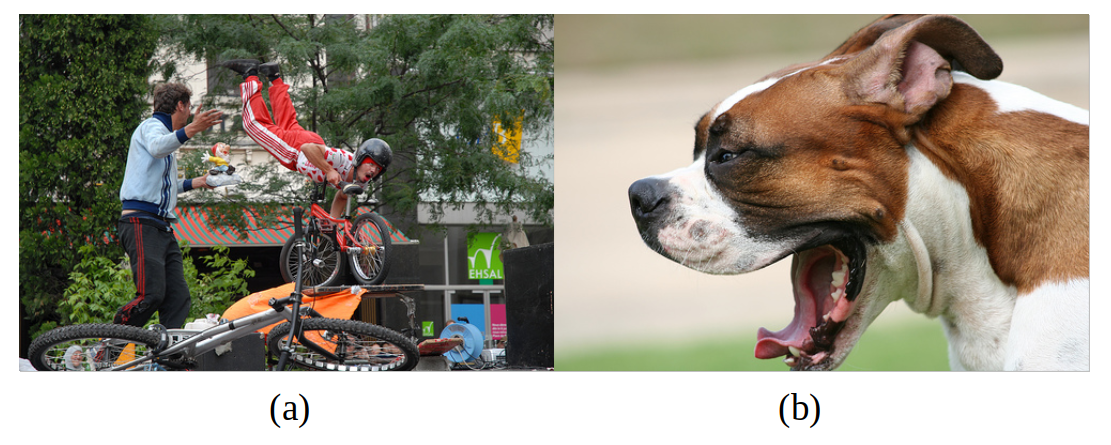
\includegraphics[width=0.8\textwidth]{long_short.jpg}
    \caption{The example images from dataset with (a)longest and (b)shortest Persian captions.} \label{fig2}
  \end{center}
\end{figure}

The shortest captions just contain two words and there are 15 captions with this length which are in the following row numbers: 5801, 6226, 6466, 12606, 13956, 18942, 19937, 25746, 32061, 34616, 38627, 41049, 42221, 44634, and 47940. One of the examples with the shortest caption length is row 34616 in csv file (see Fig.~\ref{fig2}.b):\begin{farsi}
\arabicfont\small
سگ" "خمیازه\end{farsi}
which means: ``Dog's yawn''.

In the proposed dataset, the average word counts per caption is calculated to be 12.33 words. Additionally, the standard deviation of captions lengths is determined to be 5.19. The standard deviation quantifies the extent of variability or dispersion among the caption lengths based ont eh number of words in the dataset. It provides a measure of how spread out the word lengths are from the average value, 12.33, offering insights into the distribution of word lengths and the overall diversity within the dataset (see Fig.~\ref{fig3}).

The dataset analysis shows a diverse range of word lengths in the captions, spanning from two to 77 words per caption. While no specific pattern emerged, varying frequencies of word lengths have been observed. The most frequently occurring word length was nine words, repeating a substantial number of 4808 times. Additionally, lengths 11 and 10 were also prevalent, each repeating 4730 times. Moreover, length eight was observed with a frequency of 4465 repetitions, while length 12 appeared 4201 times. These findings provide a comprehensive overview of the word length distribution within the dataset, showcasing both the range of word counts and the notable occurrences of specific lengths.

\begin{figure}
  \begin{center}
    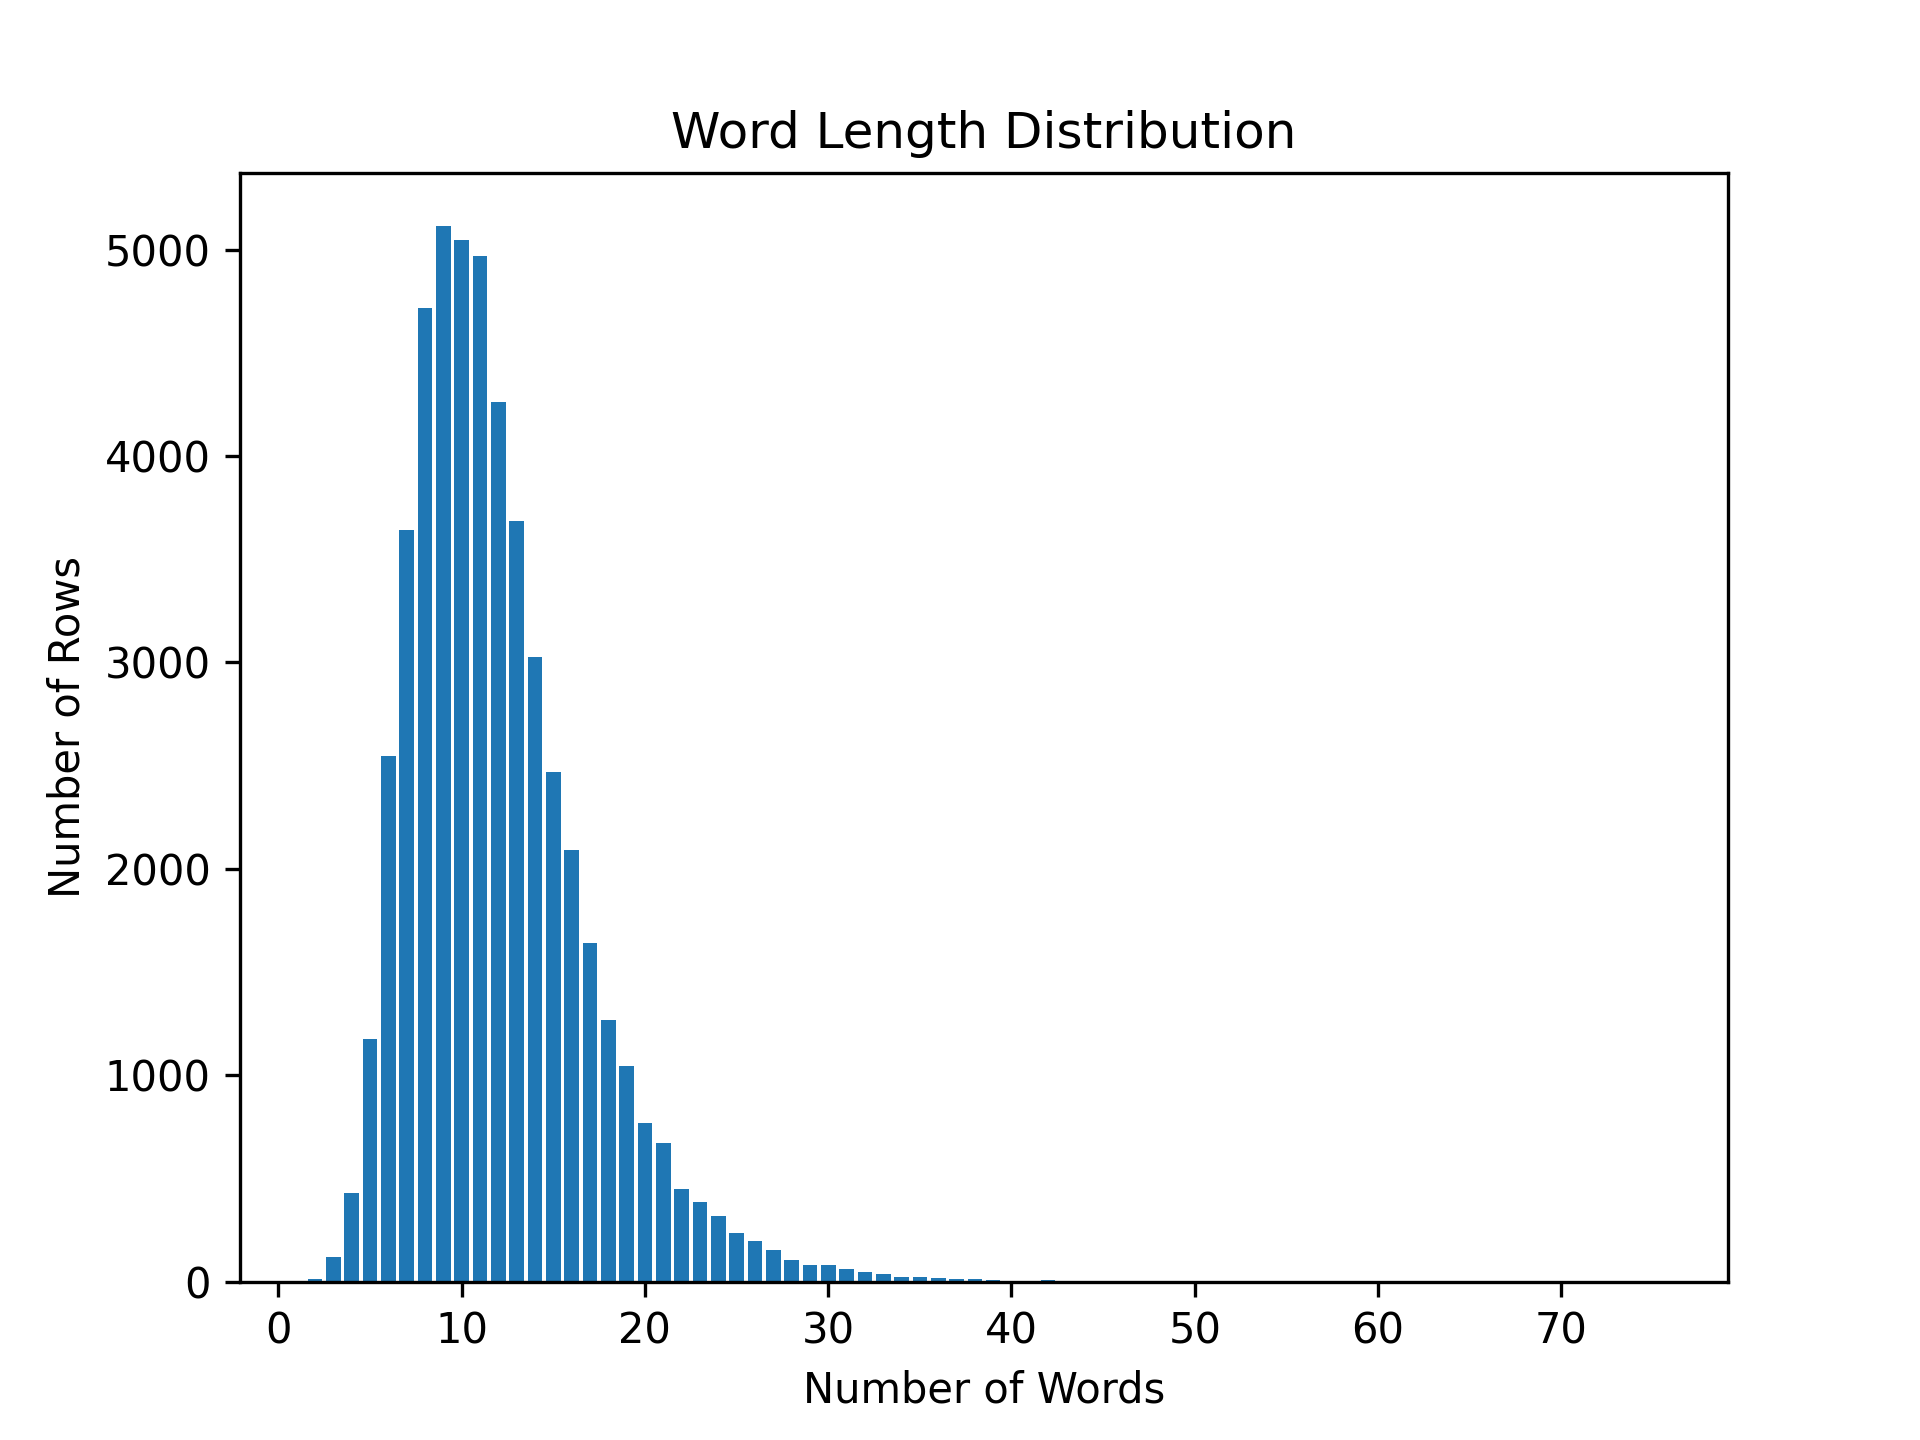
\includegraphics[width=0.6\textwidth]{length_distribution.png}
    \caption{Distribution of word lengths in captions and number of captions per word length.}
    \label{fig3}
  \end{center}
\end{figure}

In the dataset analysis, it was observed that certain words appeared with high frequency, indicating their significance in the dataset. The 10 most repeated words are as following: word \begin{farsi} \arabicfont\small "یک"\end{farsi} (a/an) appeared the most, occurring 30,100 times, suggesting its prevalence and potential importance within the context. Similarly, the word \begin{farsi} \arabicfont\small "در"\end{farsi} (in) was also highly recurrent, appearing 28,029 times. The words \begin{farsi} \arabicfont\small "با"\end{farsi} (with) and \begin{farsi} \arabicfont\small "و"\end{farsi} (and) followed closely behind with 21,102 and 20,115 occurrences, respectively, indicating their frequent usage.

Furthermore, the word \begin{farsi} \arabicfont\small "که"\end{farsi} (that) appeared 19,285 times, highlighting its significance in connecting clauses or introducing relative pronouns. The word \begin{farsi} \arabicfont\small "است"\end{farsi} (is) occurred 15,473 times, implying its role in expressing existence or attribution. The prepositions\begin{farsi} \arabicfont\small "از"\end{farsi} (from) and \begin{farsi} \arabicfont\small "را"\end{farsi} (particle for direct object) and \begin{farsi} \arabicfont\small "به"\end{farsi} (to) were also among the most repeated words, with 13,109, 9,974, and 9,615 occurrences, respectively, indicating their frequent usage to denote origin, direct object, and destination.

Additionally, the word \begin{farsi} \arabicfont\small "روی"\end{farsi} (on) appeared 8,996 times, suggesting its relevance in referring to surfaces or indicating location. These findings shed light on the prominent words in the dataset, providing valuable insights into the language patterns and themes present within the text.

\section{Experiments, Results, and Discussions}

This section presents the detailed experiment conducted to develop and evaluate the Persian Image Captioning dataset and its performance using the MobileNetV3Small image feature extractor. It starts by describing the dataset loading process, preprocessing of captions, and the dataset for training and testing. Next, it elaborates on the image feature extraction technique using the pre-trained MobileNetV3Small model. The extracted image features serve as inputs to the subsequent Persian Image Captioning model.

\subsection{Dataset Preprocessing}
The dataset is loaded using the Python pathlib module to work with file paths. The function reads the content of captions, which contains image filenames and their corresponding captions in Persian (each image have five different captions). The extracted image filename and caption pairs are stored as a list of tuples. The initial dataset have multiple captions (five captions) for each image. An one-to-one correspondence between images and captions is established, ensuring that each image now corresponds to a single caption. The final dataset contains an equal number of images and captions, enabling efficient training with a clear image-to-caption mapping.

To make it easier to access captions based on the image filename, a Python dictionary is created, which is a specialized dictionary that provides default values for keys that do not exist. In this case, the default value is an empty list. Then iterates through the list of image filename-caption tuples and appends each caption to the list associated with the corresponding image filename key in the dictionary. The content of the training and testing image-caption pairs splits into separate lines and then creates a list of image-caption tuples for both the training and testing sets. Each tuple in these lists contains the image filename and a list of its associated captions.

\textbf{Tokenization:}
The text tokenization and vectorization process aims to convert raw text captions into numerical sequences, making them suitable for further processing in the Persian Image Captioning model. The TextVectorization layer is employed to achieve this. \textbf{Standardization} is applied to each text caption to perform text. It converts all text to lowercase, removes punctuation, and adds [START] and [END] tokens to indicate the beginning and end of each caption.
\textbf{Vocabulary Creation:}
A vocabulary of the top 10000 words is computed using the TextVectorization layer. This vocabulary represents the unique words present in the captions.

\subsection{Image Feature Extractor}

After loading the dataset, an image feature extractor using the MobileNetV3Small model from TensorFlow. MobileNetV3Small is a pre-trained model on the ImageNet dataset for image classification. The final classification layer is disabled, which allows the use of the last layer of feature-maps as image features. The input shape of the images is set to (224, 224, 3).

The input images are resized to a fixed size of (224, 224, 3) to match the input shape expected by the MobileNetV3Small model. The images are then batched with a batch size of 1, resulting in a batched input format of (1, 224, 224, 3) for efficient processing during training. After image preprocessing and batch input, each image is represented as a tensor of shape (1, 7, 7, 576), containing a 7x7 grid of 576 feature maps. These extracted image features will be used to train the Persian Image Captioning model.

\subsection{Transformer-decoder architecture}

The model uses a two-layer Transformer-decoder architecture to generate descriptive captions for input images which consists of several key components: Input, Decoder, and Output. The Input part involves token embedding and positional encoding. The input is responsible for embedding the token IDs and positional information for the input text sequences combine two embeddings. First, the Token Embedding looks up the embedding vector for each token ID from the vocabulary. It uses the Embedding layer from Keras with \texttt{mask\_zero=True} to handle masking for the model. Second, the Positional Embedding looks up an embedding vector for each position in the sequence. It uses the Embedding layer with \texttt{max\_length} as the input dimension and \texttt{depth} as the output dimension. The position embeddings are learned during training, allowing the model to generalize better to longer sequences.

The decoder consists of a stack of DecoderLayers, each containing three sublayers: Causal Self-Attention, Cross Attention (to the input image), and FeedForward. This design enables the model to leverage both the image features and the generated text while generating captions.

The model performs multiclass classification over the output vocabulary to generate descriptive captions for the input images. The output layer's design is not explicitly provided in this section but typically involves a Dense layer followed by a softmax activation function to compute the probability distribution of words in the vocabulary.

\subsection{Model Specifications}

The model is a two-layer Transformer-decoder architecture. The model includes the temperature parameter, which enables interpolation between three distinct decoding modes. These modes consist of Greedy Decoding $temperature = 0.0$, Random Sampling $temperature = 1.0$, and Uniform Random Sampling $temperature > 1.0$.

Before starting the training process, the model needs to be compiled with the necessary settings. The optimizer used for training is \texttt{Adam Optimizer} Which is an extension of the stochastic gradient descent (SGD) optimization algorithm that combines the concepts of adaptive learning rates and momentum. The optmizer is used with a learning rate of $1 \times 10^{-4}$. The loss function used for optimization is  function to calculate the softmax cross-entropy loss between the true labels and the model's predicted logits. It is commonly employed in multi-class classification tasks, where the ground truth labels are represented as integers (sparse labels).

After calculating the initial loss, a mask is created to filter out certain tokens in the input sequence. The mask is constructed based on two conditions: labels != 0 and loss < $1 \mathrm{e} 8$. When calculating the loss, it is ensured to pay attention to the condition loss < $1 \mathrm{e} 8$. This step is crucial as it helps discard artificial and impossibly high losses related to banned tokens. By filtering out these infeasible losses, we ensure that the loss and accuracy computations are more reliable. The purpose of this mask is to discard tokens with a label of 0 (padding tokens) and to handle any numerical issues that might arise from very large losses. Additionally, the model is evaluated during training using the custom metric for accuracy.

The training data is passed to the model, and it is repeated indefinitely using \texttt{repeat()} to ensure enough iterations for the specified number of epochs. The \texttt{steps\_per\_epoch} parameter is set to 100, indicating the number of batches to process in one epoch. The validation data is also passed to the model for evaluation and is similarly repeated using \texttt{repeat()}. The \texttt{validation\_steps} parameter is set to 20, which specifies the number of batches to process during validation in each epoch. The total number of training epochs is set to 100. 

Additionally, to provide feedback during training, we set up a Callback. This callback is responsible for generating captions for the surfer image at the conclusion of each epoch. This way, we can observe the model's progress and evaluate the quality of the generated captions over multiple training iterations. The feedback from this callback assists us in fine-tuning the model and achieving better performance in caption generation.

\subsection{Results}

Following the completion of model training, the progression of loss Fig.~\ref{fig4}.b and accuracy  Fig.~\ref{fig4}.a throughout the training phase. The blue line corresponds to the training results, while the orange line represents the validation results.
As evident from Fig.~\ref{fig4}, the accuracy attained reaches a maximum of approximately 38\%. It is important to note that this work primarily serves as a representation of the dataset, without further optimization efforts to achieve higher accuracy. Nevertheless, the accuracy results are noteworthy considering the limited enhancements made to the model.

\begin{figure}
  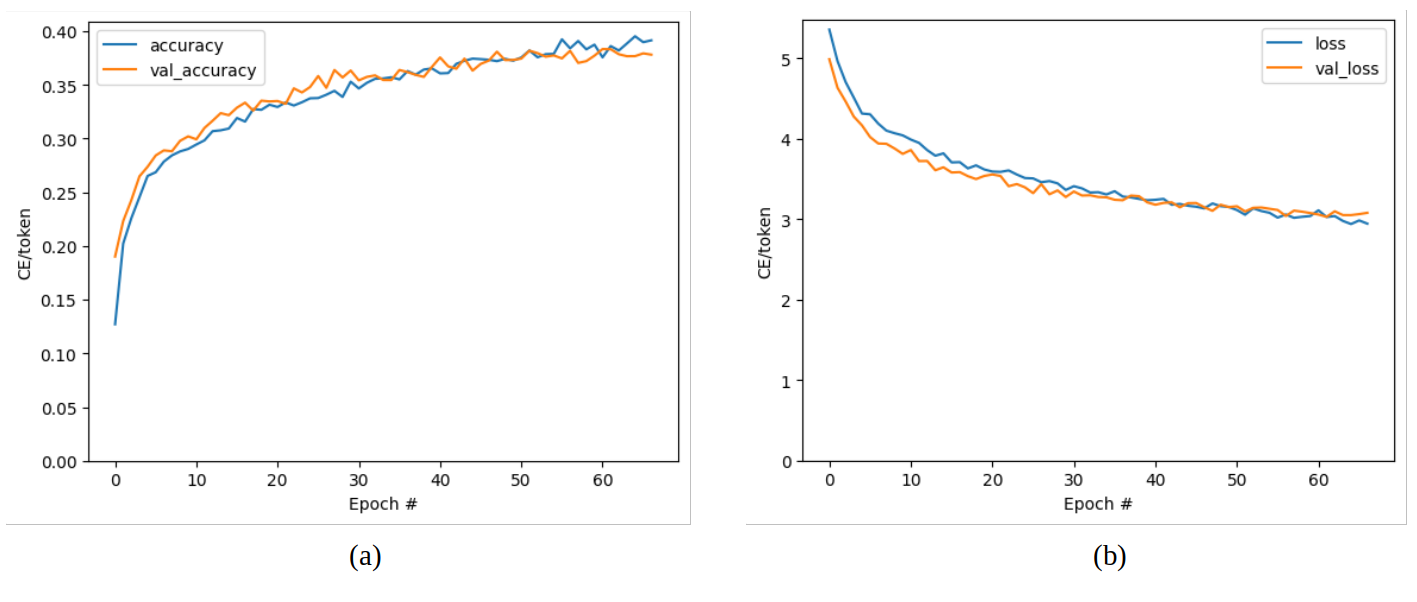
\includegraphics[width=\textwidth]{loss.png}
  \caption{Training and Validation Performance of the Model. The plot displays the changes in accuracy (a) and loss(b) during the training (blue) and validation (orange) process.} \label{fig4}
\end{figure}

Surprisingly, when examining the performance on unseen images, the generated captions are relatively satisfactory. The dataset predominantly comprises images of dogs, streets, and humans, which appears to have influenced the model's focus in caption creation. Despite the constraints, the model exhibits promising performance in generating captions relevant to these specific scenarios. In Fig.~\ref{fig5}, an intriguing example is presented, wherein the image depicts an elephant walking on wetlands. The model identifies it as a black dog which is running.The predicated caption for this image in Persian is \begin{farsi}
\arabicfont\small
 سیاه سگ یک است دویدن حال در
\end{farsi} Remarkably, despite the misclassification, the caption generated by the model exhibits impeccable grammar. The figure further includes attention maps, offering valuable insights into the word-by-word caption generation process, despite the model's misperception of the image content.

\begin{figure}
  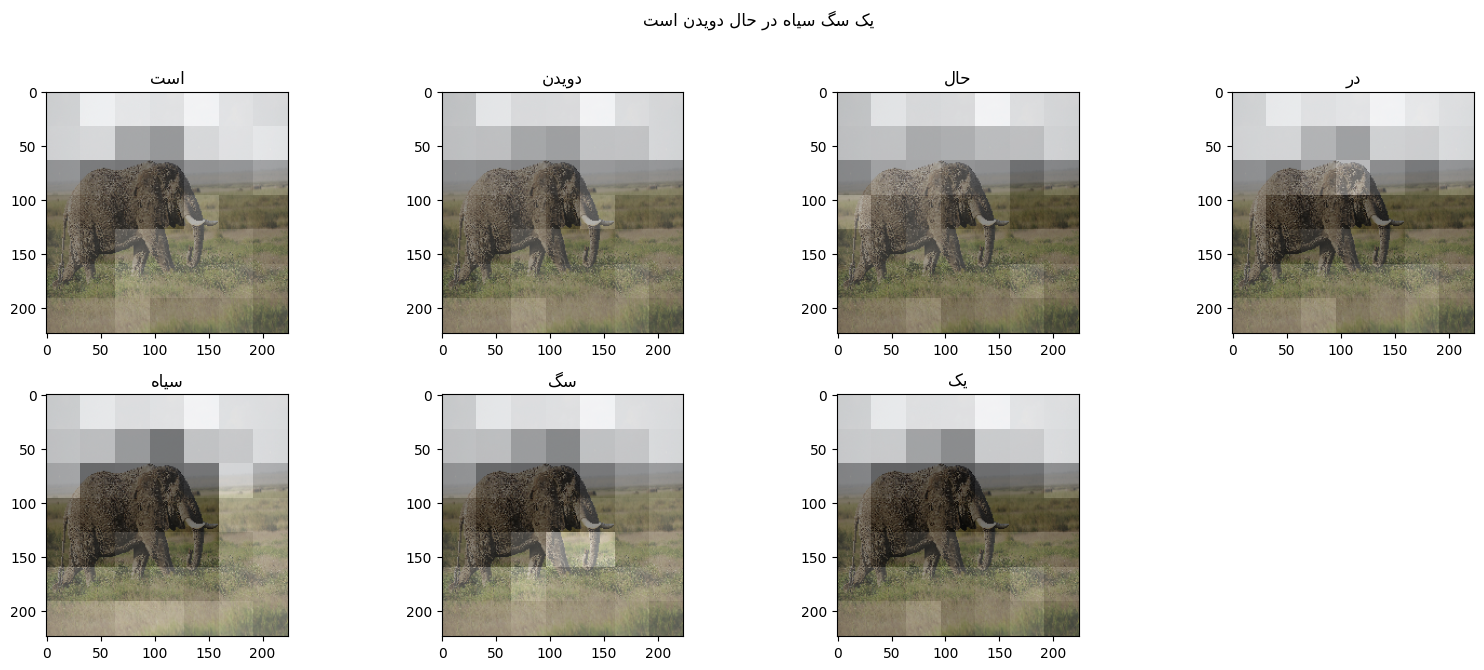
\includegraphics[width=\textwidth]{elephant.png}
  \caption{ Predicted caption and attention maps for captioning an image with an elephant walking.} \label{fig5}
\end{figure}

Furthermore, several additional examples in the dataset highlight the overall accuracy of the provided captions. However, a notable challenge arises from biased images containing specific scenes, leading to misinterpretations by the model. For instance, the model's inability to discern a train from a man or a camera from a machine illustrates the impact of scene biases on the model's comprehension. Addressing these biases becomes imperative to enhance the model's capacity for accurate image captioning in diverse real-world scenarios.

\section{Conclusion and Future Work}
In this paper, a novel dataset for image captioning presented with a specific focus on Persian annotations and sourced from Flicker30k.
In conclusion, the model employed for feature extraction is MobileNetV3Small, coupled with a two-layer transformer decoder network. Despite achieving a modest 38\% accuracy, the model consistently produces grammatically correct captions. Nevertheless, the dataset's limited real-world image representation introduces biases, hindering the model's ability to comprehend certain scenes accurately. To enhance performance, augmenting the dataset with diverse real-world images and exploring more advanced models hold promise for improving accuracy and contextual relevance in image captioning tasks.
Moving forward, our future plans involve expanding the dataset by including a larger number of images and adding multiple captions per image. This expansion aims to enhance the dataset's diversity and provide researchers with a broader range of data to explore. Additionally, we intend to categorize the images into distinct classes, such as landscapes, humans, and animals, for targeted analysis.


% ---- Bibliography ----
\begin{thebibliography}{8}
\bibitem{Karpathy2015}
Karpathy, Andrej, and Li Fei-Fei. "Deep visual-semantic alignments for generating image descriptions." Proceedings of the IEEE conference on computer vision and pattern recognition. 2015.

\bibitem{Vinyals2015}
Vinyals, Oriol, et al. "Show and tell: A neural image caption generator." Proceedings of the IEEE conference on computer vision and pattern recognition. 2015.

\bibitem{Xu2015}
Xu, Kelvin, et al. "Show, attend and tell: Neural image caption generation with visual attention." International conference on machine learning. PMLR, 2015.

\bibitem{Luo2023}
Luo, Jianjie, et al. "Semantic-conditional diffusion networks for image captioning." Proceedings of the IEEE/CVF Conference on Computer Vision and Pattern Recognition. 2023.

\bibitem{MSCOCO}
Lin, Tsung-Yi, et al. "Microsoft coco: Common objects in context." Computer Vision–ECCV 2014: 13th European Conference, Zurich, Switzerland, September 6-12, 2014, Proceedings, Part V 13. Springer International Publishing, 2014.

\bibitem{Flickr8k}
Rashtchian, Cyrus, et al. "Collecting image annotations using amazon’s mechanical turk." Proceedings of the NAACL HLT 2010 workshop on creating speech and language data with Amazon’s Mechanical Turk. 2010.

\bibitem{Flickr30k}
Young, Peter, et al. "From image descriptions to visual denotations: New similarity metrics for semantic inference over event descriptions." Transactions of the Association for Computational Linguistics 2 (2014): 67-78.

\bibitem{Multi30k}
Elliott, Desmond, et al. "Multi30k: Multilingual english-german image descriptions." arXiv preprint arXiv:1605.00459 (2016).

\bibitem{Xue}
Xue, Linting, et al. "mT5: A massively multilingual pre-trained text-to-text transformer." arXiv preprint arXiv:2010.11934 (2020).

\bibitem{Zoph}
Zoph, Barret, and Kevin Knight. "Multi-source neural translation." arXiv preprint arXiv:1601.00710 (2016).

\bibitem{Rosa}
Rosa, Guilherme Moraes, et al. "A cost-benefit analysis of cross-lingual transfer methods." arXiv preprint arXiv:2105.06813 (2021).

\bibitem{VIST}
Huang, Ting-Hao, et al. "Visual storytelling." Proceedings of the 2016 conference of the North American chapter of the association for computational linguistics: Human language technologies. 2016.

\bibitem{Nocaps}
Agrawal, Harsh, et al. "Nocaps: Novel object captioning at scale." Proceedings of the IEEE/CVF international conference on computer vision. 2019.

\bibitem{Openimages}
Krasin, Ivan, et al. "Openimages: A public dataset for large-scale multi-label and multi-class image classification." Dataset available from https://github. com/openimages 2.3 (2017): 18.

\bibitem{VizWiz}
Gurari, Danna, et al. "Captioning images taken by people who are blind." Computer Vision–ECCV 2020: 16th European Conference, Glasgow, UK, August 23–28, 2020, Proceedings, Part XVII 16. Springer International Publishing, 2020.

\bibitem{Korean}
Jeong, Changhoon, et al. "Korean tourist spot multi-modal dataset for deep learning applications." Data 4.4 (2019): 139.

\bibitem{ImageCLEF2018}
Ionescu, Bogdan, et al. "Overview of ImageCLEF 2018: Challenges, datasets and evaluation." Experimental IR Meets Multilinguality, Multimodality, and Interaction: 9th International Conference of the CLEF Association, CLEF 2018, Avignon, France, September 10-14, 2018, Proceedings 9. Springer International Publishing, 2018.

\end{thebibliography}
\end{document}
